% LaTeX source for ``Introduction to Computer Science (Python Edition)''
% Copyright (c) 2021- David S. Read, All Rights Reserved
% Built upon, ``Python for Informatics: Exploring Information''
% Copyright (c)  2010-  Charles R. Severance, All Rights Reserved

\chapter{Iteration}
\index{iteration}
\index{loop}

\section{Updating variables}
\label{update}

\index{update}
\index{variable!updating}

A common pattern in assignment statements is an assignment statement
that updates a variable -- 
where the new value of the variable depends on the old.

\beforeverb
\begin{verbatim}
x = x + 1
\end{verbatim}
\afterverb
%
This means ``get the current value of {\tt x}, add 1, and then
update {\tt x} with the new value.''

If you try to update a variable that doesn't exist, you get an
error, because Python evaluates the right side before it assigns
a value to {\tt x}:

\beforeverb
\begin{verbatim}
>>> x = x + 1
NameError: name 'x' is not defined
\end{verbatim}
\afterverb
%
Before you can update a variable, you have to {\bf initialize}
it, usually with a simple assignment:

\index{initialization (before update)}

\beforeverb
\begin{verbatim}
>>> x = 0
>>> x = x + 1
\end{verbatim}
\afterverb
%
Updating a variable by adding 1 is called an {\bf increment};
subtracting 1 is called a {\bf decrement}.

\index{increment}
\index{decrement}

\section{The {\tt while} statement}

\index{statement!while}
\index{while loop}
\index{loop!while}
\index{iteration}

Computers are often used to automate repetitive tasks.  Repeating
identical or similar tasks without making errors is something that
computers do well and people do poorly.
Because iteration is so common, Python provides several
language features to make it easier.  

One form of iteration in Python is the {\tt while} statement.  Here is 
a simple program that counts down from five and then says ``Blastoff!''.

\beforeverb
\begin{verbatim}
n = 5
while n > 0:
    print(n)
    n = n - 1
print('Blastoff!')
\end{verbatim}
\afterverb
%
You can almost read the {\tt while} statement as if it were English.
It means, ``While {\tt n} is greater than 0,
display the value of {\tt n} and then reduce the value of
{\tt n} by 1.  When you get to 0, exit the {\tt while} statement and
display the word {\tt Blastoff!}''

\beforefig
\centerline{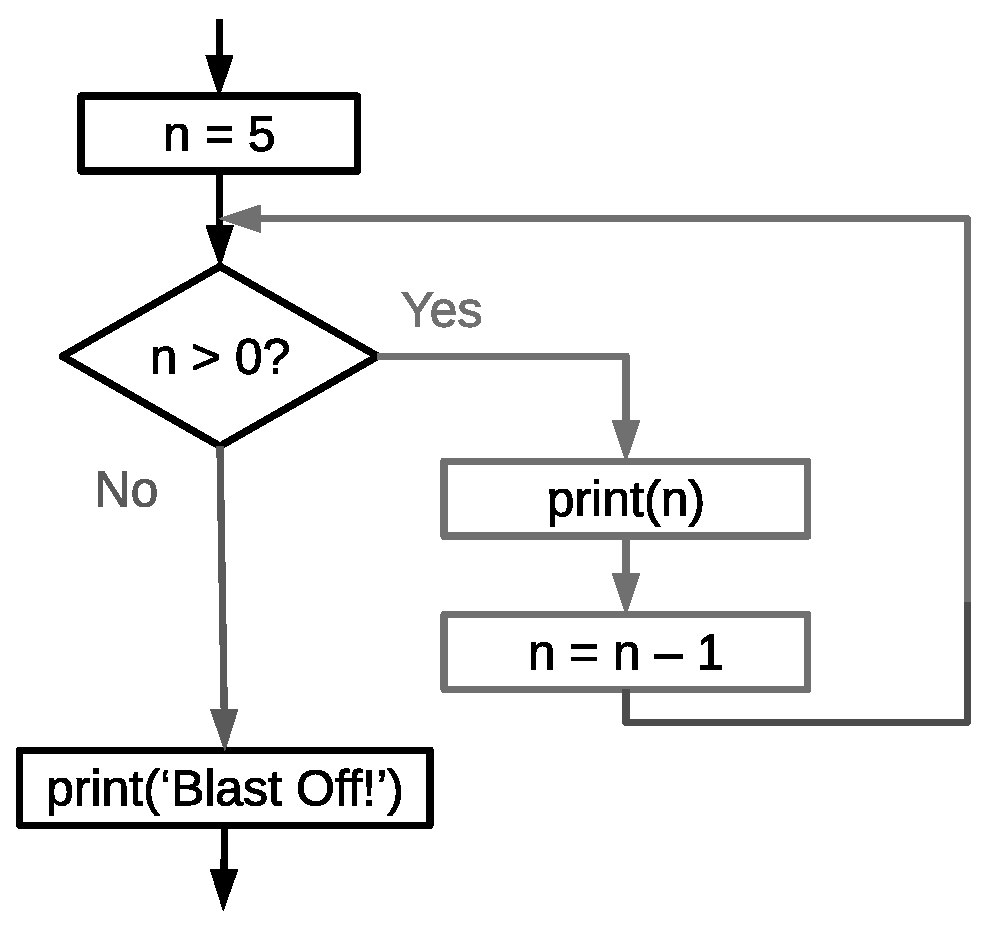
\includegraphics[height=3in]{figs2/while.eps}}
\afterfig

\index{flow of execution}

More formally, here is the flow of execution for a {\tt while} statement:

\begin{enumerate}

\item Evaluate the condition, yielding {\tt True} or {\tt False}.

\item If the condition is false, exit the {\tt while} statement
and continue execution at the next statement.

\item If the condition is true, execute the
body and then go back to step 1.

\end{enumerate}

This type of flow is called a {\bf loop} because the third step
loops back around to the top.  We call each time we execute the body of 
the loop an {\bf iteration}.  For the above loop, we 
would say, ``It had five iterations'', which means that the body of
the loop was executed five times.

\index{condition}
\index{loop}
\index{body}

The body of the loop should change the value of one or more variables
so that eventually the condition becomes false and the loop
terminates.  
We call the variable that changes each time the loop
executes and controls when the loop finishes the 
{\bf iteration variable}.
If there is no iteration variable, the loop will repeat forever, 
resulting in an {\bf infinite loop}.  

\section{Infinite loops}

An endless source of amusement for 
programmers is the observation that the directions on shampoo,
``Lather, rinse, repeat,'' are an infinite loop because 
there is no {\bf iteration variable} telling you how many times
to execute the loop.

\index{infinite loop}
\index{loop!infinite}

In the case of {\tt countdown}, we can prove that the loop
terminates because we know that the value of {\tt n} is finite, and we
can see that the value of {\tt n} gets smaller each time through the
loop, so eventually we have to get to 0.  Other times a loop is obviously
infinite because it has no iteration variable at all.

\section{``Infinite loops'' and {\tt break}}
\index{break statement}
\index{statement!break}

Sometimes you don't know it's time to end a loop until you get half
way through the body.  In that case you can write an infinite loop on purpose
and then use the {\tt break} statement to jump out of the loop.

This loop is obviously an {\bf infinite loop} because the logical 
expression on the
{\tt while} statement is simply the logical constant {\tt True}:

\beforeverb
\begin{verbatim}
n = 10
while True:
    print(n) 
    n = n - 1
print('Done!')
\end{verbatim}
\afterverb
%
If you make the mistake and run this code, you will learn quickly how
to stop a runaway Python process on your system or find where the power-off
button is on your computer.  
This program will 
run forever or until your battery runs out 
because the logical expression at the top of the loop 
is always true by virtue of the fact that the expression is the 
constant value {\tt True}.

While this is a dysfunctional infinite loop, we can still use this pattern
to build useful loops as long as we carefully add code to the 
body of the loop to explicitly exit the loop using {\tt break} 
when we have reached 
the exit condition.

For example, suppose you want to take input from the user until they
type {\tt done}.  You could write:

\beforeverb
\begin{verbatim}
while True:
    line = input('> ')
    if line == 'done':
        break
    print(line)
print('Done!')
\end{verbatim}
\afterverb
%
The loop condition is {\tt True}, which is always true, so the
loop runs repeatedly until it hits the break statement.

Each time through, it prompts the user with an angle bracket.
If the user types {\tt done}, the {\tt break} statement exits
the loop.  Otherwise the program echoes whatever the user types
and goes back to the top of the loop.  Here's a sample run:

\beforeverb
\begin{verbatim}
> hello there
hello there
> finished
finished
> done
Done!
\end{verbatim}
\afterverb
%
This way of writing {\tt while} loops is common because you
can check the condition anywhere in the loop (not just at the
top) and you can express the stop condition affirmatively
(``stop when this happens'') rather than negatively (``keep going
until that happens.'').

\section{Finishing iterations with {\tt continue}}
\index{continue statement}
\index{statement!continue}

Sometimes you are in an iteration of a loop and want to finish the
current iteration and immediately jump to the next iteration.
In that case you can use the {\tt continue}
statement to skip to the next iteration without finishing the
body of the loop for the current iteration.

Here is an example of a loop that copies its input until the user
types ``done'', but treats lines that start with the hash character
as lines not to be printed (kind of like Python comments).

\beforeverb
\begin{verbatim}
while True:
    line = input('> ')
    if line[0] == '#' :
        continue
    if line == 'done':
        break
    print(line)
print('Done!')
\end{verbatim}
\afterverb
%
Here is a sample run of this new program with {\tt continue} added.

\beforeverb
\begin{verbatim}
> hello there
hello there
> # don't print this
> print this!
print this!
> done
Done!
\end{verbatim}
\afterverb
%
All the lines are printed except the one that starts with the hash
sign because when the {\tt continue} is executed, it ends 
the current iteration and jumps
back to the {\tt while} statement to start the next iteration, thus 
skipping the {\tt print} statement.

\section{A word of caution}
There is debate among programmers about the use of the {\tt break} and
{\tt continue} statements. Some programmers consider these statements as useful for
writing concise code. Other programmers dislike using these statements and think that
they lead to code that is difficult to read and prone to bugs. A general guideline is
to use the {\tt break} and {\tt continue} statements in loops that are short and simple, 
and to use other approaches for loop control in longer or more complex loops. Your goal 
is to write code that is easy for others to quickly read and understand.

An additional iteration variable is an alternative to using a {\tt break} statement.
An {\tt if} statement can be used in place of a {\tt continue} statement. For example, here 
is the code from above rewritten without using {\tt break} or {\tt continue}.

\beforeverb
\begin{verbatim}
line = input('> ')
while line != 'done':
    if line[0] != '#':
        print(line)
    line = input('> ')
print('Done!')
\end{verbatim}
\afterverb

\section{Definite loops using {\tt for} }
\index{for statement}
\index{statement!for}

Sometimes we want to loop through a {\bf collection} of things such 
as a list of words, the lines in a file, or a list of numbers.
When we have a list of things to loop through, we can
construct a \emph{definite} loop using a {\tt for} statement.
We call the {\tt while} statement an \emph{indefinite} loop
because it simply loops until some condition becomes {\tt False}, 
whereas the {\tt for} loop is looping through a known
collection of items so it runs through as many iterations as there
are items in the collection.

The syntax of a {\tt for} loop is similar to the {\tt while} loop
in that there is a {\tt for} statement and a loop body:

\beforeverb
\begin{verbatim}
friends = ['Joseph', 'Glenn', 'Sally']
for friend in friends:
    print('Happy New Year:', friend)
print('Done!')
\end{verbatim}
\afterverb
%
In Python terms, 
the variable {\tt friends} is a list\footnote{We will 
examine lists in more detail in a later chapter.} 
of three strings and the {\tt for}
loop goes through the list and executes the body once
for each of the three strings in the list resulting in this output:

\beforeverb
\begin{verbatim}
Happy New Year: Joseph
Happy New Year: Glenn
Happy New Year: Sally
Done!
\end{verbatim}
\afterverb
%

Translating this {\tt for} loop to English is not as direct as the 
{\tt while}, but if you think of friends as a {\bf collection},
it goes like this: ``Run the statements in the body of the 
for loop once for each friend \emph{in} the collection named {\tt friends}.''

Looking at the {\tt for} loop, {\bf for} and {\bf in} are reserved
Python keywords, and {\tt friend} and {\tt friends} are variables.

{\tt {\bf for} friend {\bf in} friends{\bf :}\\
\verb"    "{\bf print(} 'Happy New Year', friend {\bf )}}

In particular, {\tt friend} is the {\bf iteration variable} for 
the {\tt for} loop.  The variable {\tt friend} changes for each iteration of
the loop and controls when the {\tt for} loop completes.  The 
{\bf iteration variable} steps successively through the 
three strings stored in the {\tt friends} variable.


\section{Loop patterns}

Often we use a {\tt for} or {\tt while} loop to go through a list of items
or the contents of a file and we are looking for something such as
the largest or smallest value of the data we scan through.

These loops are generally constructed by:

\begin{itemize}

\item Initializing one or more variables before the loop starts

\item Performing some computation on each item in the loop body, 
possibly changing the variables in the body of the loop

\item Looking at the resulting variables when the loop completes

\end{itemize}

We will use a list of numbers to demonstrate the concepts and construction
of these loop patterns.  

\subsection{Counting and summing loops}

For example, to count the number of items
in a list, we would write the following {\tt for} loop:

\beforeverb
\begin{verbatim}
count = 0
for itervar in [3, 41, 12, 9, 74, 15]:
    count = count + 1
print('Count: ', count)
\end{verbatim}
\afterverb
%
We initialize the variable {\tt count} to zero before the loop starts,
then we write a {\tt for} loop to run through the list of numbers.
Our {\bf iteration} variable is named {\tt itervar} and while we do
not use {\tt itervar} in the loop, it does control the loop and cause
the loop body to be executed once for each of the values in the list.

In the body of the loop, we add 1 to the current value of {\tt count}
for each of the values in the list.  While the loop is executing, the 
value of {\tt count} is the number of values we have seen ``so far''.

Once the loop completes, the value of {\tt count} is the total number
of items.   The total number ``falls in our lap'' at the end of the 
loop.  We construct the loop so that we have what we want when the loop
finishes.

Another similar loop that computes the total of a collection of numbers
is as follows:

\beforeverb
\begin{verbatim}
total = 0
for itervar in [3, 41, 12, 9, 74, 15]:
    total = total + itervar
print('Total: ', total)
\end{verbatim}
\afterverb
%
In this loop we \emph{do} use the {\bf iteration variable}.
Instead of simply adding one to the {\tt count} as in the previous loop, 
we add the actual number (3, 41, 12, etc.) to the running 
total during each loop iteration.
If you think about the variable {\tt total}, it contains the 
``running total of the values so far''.  So before the loop
starts {\tt total} is zero because we have not yet seen any values,
during the loop {\tt total} is the running total, and at the end of 
the loop {\tt total} is the overall total of all the values 
in the list.

As the loop executes, {\tt total} \emph{accumulates} the sum of the
elements; a variable used this way is sometimes called an
{\bf accumulator}.
\index{accumulator!sum}

Neither the counting loop nor the summing loop are particularly 
useful in practice because there are built-in functions 
{\tt len()} and {\tt sum()} that compute the number of 
items in a list and the total of the items in the list
respectively.

\subsection{Maximum and minimum loops}

\index{loop!maximum}
\index{loop!minimum}
\index{None special value}
\index{special value!None}
\label{maximumloop}
To find the largest value in a collection such as a list, we construct the
following loop:

\beforeverb
\begin{verbatim}
largest = None
print 'Before:', largest
for itervar in [3, 41, 12, 9, 74, 15]:
    if largest is None or itervar > largest :
        largest = itervar
    print('Loop:', itervar, largest)
print('Largest:', largest)
\end{verbatim}
\afterverb
%
When the program executes, the output is as follows:

\beforeverb
\begin{verbatim}
Before: None
Loop: 3 3
Loop: 41 41
Loop: 12 41
Loop: 9 41
Loop: 74 74
Loop: 15 74
Largest: 74
\end{verbatim}
\afterverb
%
The variable {\tt largest} is best thought of as 
the ``largest value we have seen so far''.
Before the loop, we initialize {\tt largest} to the constant {\tt None}.  
{\tt None} is a special constant value which we can 
store in a variable to mark 
the variable as ``empty''.  

Before the loop starts, the largest value we have seen so far 
is {\tt None} since we have not yet seen any values.  While the 
loop is executing, if {\tt largest} is {\tt None} then we take
the first value we see as the largest so far.   You can see in 
the first iteration when the value of {\tt itervar} is 3,
since {\tt largest} is {\tt None}, we immediately update 
{\tt largest} to be 3.

After the first iteration, {\tt largest} is no longer {\tt None},
so the second part of the compound logical expression that checks
{\tt itervar > largest} triggers only when we see a value that is
larger than the ``largest so far''.  When we see a new ``even larger''
value we take that new value for {\tt largest}.  You can see in the 
program output that {\tt largest} progresses from 3 to 41 to 74.

At the end of the loop, we have scanned all of the values and
the variable {\tt largest} now does contain the largest value
in the list.

To compute the smallest number, the code is very similar with one
small change:

\beforeverb
\begin{verbatim}
smallest = None
print 'Before:', smallest
for itervar in [3, 41, 12, 9, 74, 15]:
    if smallest is None or itervar < smallest:
        smallest = itervar
    print('Loop:', itervar, smallest)
print('Smallest:', smallest)
\end{verbatim}
\afterverb
%
Again, {\tt smallest} is the ``smallest so far'' before, during, and after the 
loop executes.  When the loop has completed, {\tt smallest} contains the
minimum value in the list.

Again as in counting and summing, the built-in functions 
{\tt max()} and {\tt min()} make writing these exact loops
unnecessary.

The following is a simple version of the Python built-in
{\tt min()} function:

\beforeverb
\begin{verbatim}
def min(values):
    smallest = None
    for value in values:
        if smallest is None or value < smallest:
            smallest = value
    return smallest
\end{verbatim}
\afterverb
%
In the function version of the smallest code, we removed all of the 
{\tt print} statements so as to be equivalent to the {\tt min} 
function which is already built in to Python.

\section{Debugging}

As you start writing bigger programs, you might find yourself
spending more time debugging.  More code means more chances to
make an error and more places for bugs to hide.

\index{debugging!by bisection}
\index{bisection, debugging by}

One way to cut your debugging time is ``debugging by bisection.''
For example, if there are 100 lines in your program and you
check them one at a time, it would take 100 steps.

Instead, try to break the problem in half.  Look at the middle
of the program, or near it, for an intermediate value you
can check.  Add a {\tt print} statement (or something else
that has a verifiable effect) and run the program.

If the mid-point check is incorrect, the problem must be in the
first half of the program.  If it is correct, the problem is
in the second half.

Every time you perform a check like this, you halve the number
of lines you have to search.  After six steps (which is much
less than 100), you would be down to one or two lines of code,
at least in theory.

In practice it is not always clear what
the ``middle of the program'' is and not always possible to
check it.  It doesn't make sense to count lines and find the
exact midpoint.  Instead, think about places
in the program where there might be errors and places where it
is easy to put a check.  Then choose a spot where you
think the chances are about the same that the bug is before
or after the check.

\section{Glossary}

\begin{description}

\item[accumulator:] A variable used in a loop to add up or
accumulate a result.
\index{accumulator}

\item[counter:] A variable used in a loop to count the number
of times something happened.  We initialize a counter to 
zero and then increment the counter each time we want to
``count'' something.
\index{counter}

\item[decrement:] An update that decreases the value of a variable.
\index{decrement}

\item[initialize:] An assignment that gives an initial value to
a variable that will be updated.

\item[increment:] An update that increases the value of a variable
(often by one).
\index{increment}

\item[infinite loop:] A loop in which the terminating condition is
never satisfied or for which there is no terminating condition.
\index{infinite loop}

\item[iteration:] Repeated execution of a group of statements using
either a function that calls itself or a loop.
\index{iteration}

\end{description}


\section{Exercises}

\begin{ex}
Write a program which repeatedly reads numbers until the user
enters ``done''.
Once ``done'' is entered, print out the total, count, and average
of the numbers.  If the user enters anything other than a number, 
detect their mistake using {\tt try} and {\tt except} and 
print an error message and skip to the next number.

\begin{verbatim}
Enter a number: 4
Enter a number: 5
Enter a number: bad data
Invalid input
Enter a number: 7
Enter a number: done
16 3 5.33333333333
\end{verbatim}
\end{ex}

\begin{ex}
Write another program that prompts for a list of numbers as above
and at the end prints out both the maximum and minimum of the numbers instead of the average.
\end{ex}


